%! Author = Justus Benedict Siegert
%! Date = 22.01.2023

% Preamble
\documentclass[a4paper,10pt]{scrartcl}

\bibliographystyle{plain}

% Packages
\usepackage[utf8]{inputenc}
\usepackage[ngerman]{babel}
\usepackage[T1]{fontenc}
\usepackage[normalem]{ulem}
\usepackage{wasysym}
\usepackage{graphicx}
\useunder{\uline}{\ul}{}


% Document
\begin{document}
    \title{Lucky Thirteen}
    \author{Justus Benedict Siegert}
    \date{8445024, s222312@student.dhbw-mannheim.de}
    \maketitle
    \tableofcontents
    \newpage


    \section{Einleitung}\label{sec:einleitung}
    Das Verschlüsseln von Daten ist seit der Nutzung des Internets ein wichtiges Anliegen der Nutzenden.
    Das am häufigsten genutzte Protokoll ist das Transport Layer Security Protokoll (TLS).
    Lucky 13 ist eine kryptografische Schwachstelle des TLS-Protokolls in der Version 1.1, sowie dem Vorgänger TLS 1.0, SSL, die Maßnahmen gegen Padding Oracle Attacks enthalten und dem Datagram Transport Layer Security (DTLS)~\cite[S.2]{AlFardan2013},
    bei dem die Daten kompromittiert werden.
    Durch die Schwachstelle können Angreifer Daten ausspionieren, die verschlüsselt sind und vermeintlich sicher seien.
    Die Sicherheitslücke wurde 2013 von den Wissenschaftlern Nadhem J. AlFardan and Kenneth G. Paterson, der Security Group der Royal Holloway University of London entdeckt.
    \newline
    Der Lucky 13 Angriff ist eine Art von Man in the Middle attack verbunden mit einer Padding Oracle Attack, weil der Angreifer zwischen den Client und Server muss, um die verschlüsselten Nachrichten zu lesen und zu senden.
    Gleichzeitig beruht der Angriff auf einem Padding Oracle Attack, wo verschiedene Paddings an ein Server geschickt werden, um das richtig formatierte zu erfahren.
    Dabei ist das Problem, dass das Padding nach der Berechnung des message authentication code (MAC) hinzugefügt wird und somit unauthentifizierte Daten im verschlüsselten Klartext bildet.
    Im Folgendem werden verschiedene Aspekte zum verständnis der Sicherheitslücke ausgeführt.

    \subsection{Man-in-the-Middle-Attack}\label{subsec:man-in-the-middle-attack}
    Eine Man-in-the-Middle-Attack (MITM) ist ein Angriff, bei dem eine dritte Partei eine vermeintlich direkte Verbindung von zwei anderen zwischen schaltet.
    Bei einem solchen Angriff, wird unerlaubt auf den Datenverkehr zweier Kommunikationspartner zugegriffen, in dem der Angreifer versucht zwischen den Datenverkehr der beiden Kommunikationspartner zu gelangen und diesen abzufangen oder zu manipuliert.
    Die Gefahr dabei ist, dass es nicht im Rahmen einer normalen Datenübertragung zu erkennen ist, wenn jemand sich dazwischen geschaltet hat.
    %eleg unsichere aussage

    \subsection{Padding Oracle aAttack}\label{subsec:padding-oracle-attack}
    Die Padding Oracal Attck wurde 2002 von Vaudenay entdeckt und dient als Basis für diesen Angriff.
    Bei einem Padding Oracle Attack wird ausgenutzt, dass einige Chiffren ein Padding benötigen, um eine Blockverschlüsslung durchzuführen, damit die Nachricht auf Blocklänge ist.
    Der Angreifer schickt dann Nachrichten an den Server mit verschiedenen Paddings und schaut, ob der Server das Padding akzeptiert.
    Bei einem korrektem Padding kann dann die Nachricht genutzt werden, um die Verschlüsslung der Datenpakete zu brechen.
    Durch die präzise Antwort des Servers, dass es zu einem Entschlüsselungsfehler kam, resultiert der name Orakel\cite{Rizzo2010}.
    Um den gewöhnlichen Angriff zu verhindern, wurden die Server so konfiguriert, dass allgemein nur eine Fehlerrückmeldung gesendet wird, die nicht auf die Art des Fehlers schließen lässt.
    \newline
    Bei dem Beispiel Paper von Nadhem J. AlFardan and Kenneth G. Paterson haben sie lediglich die Padding Oracle Attack in verbindung der Blockchiffre CBC verwendet.
    Dies ist ein typisches Beispiel für einen Verschlüsselungsalgorithmus, bei dem der Angriff möglich ist.


    \section{(Datagram) Transport Layer Security}\label{sec:(d)tls}
    Der vorgänger von TLS, Secure Socket Layer (SSL) 1.0 erschien im Jahr 1994, neun Monate nach der ersten Mosaic version.
    In den folgenden zwei Jahre wurden zwei weiter Versionen entwickelt und dann SSL in TLS 1.0 umbenannt.
    \newline
    TLS besteht aus zwei Hauptkomponenten: dem TLS Handshake, der für den sicheren Schlüsselaustausch zwischen dem Client und dem Server zuständig ist,
    und dem TLS Record, dieser verwendet die beim Handshake ausgehandelten Schlüssel, um eine sichere Datenübertragung zu ermöglichen.
    Die Daten werden verschlüsselt und mit einem MAC gegen manipulation geschützt.
    Die grundlegende Funktionsweise besteht darin, dass der Client eine Verbindung mit dem Server aufbaut, welcher sich mit einem Zertifikat authentifiziert.
    Der Client überprüft die Vertrauenswürdigkeit und vergleicht die Daten des Zertifikats, mit den des Servers.
    \newline
    DTLS basiert auf TLS, kann aber im Gegensatz zu TLS auch Transportprotokolle wie UDP übertragen, hat aber grundlegend dieselben Eigenschaften und Sicherheitsmerkmale

    \subsection{Cipher Block Chaining Mode Mode}\label{subsec:cbc-mode}
    Cipher Block Chaining Mode (CBC) ist eine Betriebsart in der Blockchiffre, dabei wird vor dem Verschlüsseln des Klartextblocks dieser mit dem vorausgehenden verschlüsselten Block per XOR verknüpft\ref{CBC_Mode}.
    Die Vorteiler dieses Modus sind, dass gleich Klartextblöcke unterschiedliche verschlüsselte Blöcke ergibt, allerdings können so nicht gleichzeit mehrere Blocks verschlüsselt werden, da sie von einander abhängen.
    Im weiteren Verlauf wird unter dem CBC-Mode beschrieben.
    \begin{figure}[h]
        \begin{center}
            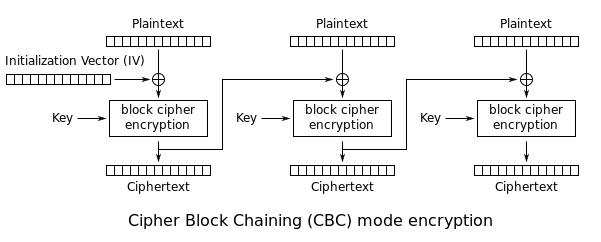
\includegraphics[width=12cm]{./Literatur/documents/wo8Bl}\newline\caption{Verschlüsselung im CBC-Mode}
            \label{CBC_Mode}
        \end{center}
    \end{figure}


    \section{Voraussetzungen für einen Angriff}\label{sec:voraussetzungen-fur-einen-angriff}
    Damit der Angriff gelingt, muss die TLS version 1.1 oder eine ältere Version mit Maßnahmen gegen Padding Oracle Attacks.
    Der Angriff ist darauf ausgelegt die Maßnahmen gegen einen normale Padding Oracle Attack zu umgehen, indem die Padding-Überprüfung beim Server nicht über den Inhalt der Antwort analysiert wird, sondern über die Verarbeitungszeit.
    Bei anderen älteren Versionen ist der Angriff deshalb nicht Empfehlenswert, weil es andere einfachere Sicherheitslücken zum Ausnutzen gibt.
    \newline
    Lucky 13 nutzt den Zeitkanal aus, welche nur getestet wurde im Lokalen Netzwerk des Servers.
    Um eine genaue Zeitmessung zu ermöglichen, muss man das Rauschen des Netzwerks analysieren, damit man die Antwortdauer der Pakete unterscheiden kann.
    Außerhalb dieses Netzwerks sind andere Variablen, die die Zeit beeinflussen und deshalb bisher nicht getestet wurden von in dem Paper der Sicherheitswissenschaftler\cite[S. 11]{AlFardan2013}.
    Des Weiteren muss man zwischen den Client und Server gelangen, um die Pakete abzufangen und an die Sequenznummern zu kommen, da diese inkrementiert wird.


    \section{Angriffsverlauf}\label{sec:angriffsverlauf}
    Der Angriff ist gleich aufgebaut wie ein normaler Padding Oracle Attack, nur dass statt die Antwort des Servers, die Antwortzeit ausschlaggebend ist für die analyse.
    Dieser Unterschied entsteht dadurch, dass bei korrekten Paddings eine MAC prüfung durchgeführt werden muss und bei falschen nicht.
    Ein Problem des Angriffs ist, dass Fehler bei TLS immer fatal sind und zu einem session abbruch führen, beidem alle Schlüssel sowie kryptografisches Material entsorgt werden.
    Bei DTLS kann ein solcher Fehler auch als nicht sehr schwerwiegend eingestuft werden, weshalb es zu keinem Abbruch der Verbindung kommt \cite[S.5]{AlFardan2013}.
    Deshalb wird zur Anfrage für die Zeitmessung immer ein DTLS Heartbeat geschickt, damit dieser Analysiert werden kann.

    \subsection{Aufbau der TLS Nachricht}\label{subsec:aufbauder-tls-nachricht}
    Zur Bildung der Nachricht wird von den genau 13 Byte (8 Byte Sequenznummer (SQN); 2 Byte Version, 1 Byte Typ, 2 Byte Länge (HDR)) und der Inhalt der Nachricht der Message Authentication Code gebildet.
    Dieser kann je nach Hashalgorithmus verschiedene Längen (16 bei HMAC-MD5, 20 bei HMAC-SHA-1 oder 32 Byte bei HMAC-SHA-256) annehmen und wir nennen ihn T\@.
    Der Inhalt (R), der MAC (T) und ein Padding (pad) werden dann mit einer Blockchiffre verschlüsselt.
    Das Padding wird so gewählt, dass die Gesamtlänge von R||T||pad gleich der Blocklänge der Chiffre ist.
    Bei 3DES beträgt die Blocklänge 8 und bei AES 16 Byte.
    Das Padding besteht aus n Byte mit dem Wert von (n-1), dadurch entstehen Paddings wie \("0\)x\(00"\), \("0\)x01||0x\(01"\) oder \("0\)x02||0x02||0x\(02"\).
    Die fertige TLS-Nachricht besteht dann 1.\ aus der Inhalt der nachricht 2.\ aus der Berechneten MAC und 3.\ dem Padding.
    Alle diese Teile werden dann verschlüsselt und bilden die gesamte Nachricht \cite[S.4]{AlFardan2013}.
    \newpage

    Nach dem der Aufbau der TLS Nachrichten beschrieben wurde, wird im Folgendem auf die Klartextwiederherstellung eingegangen.
    Unsere Grundannahmen sind dabei, dass es sich um den CBC-Mode handelt, dass wir eine Blocklänge von 16 haben, also AES verwenden und HMAC-SHA-1 verwendet wird,also der MAC 20 Byte groß ist.
    Außerdem wird nur TLS betrachtet, allerdings treffen die Funktionen auch auf DTLS zu \cite[s.7]{AlFardan2013}.

    \subsection{Wiederherstellung}\label{subsec:wiederherstellung}
    Die Entschlüsselung von Nachrichten beim Server findet rückwärts wie dir Verschlüsselung \ref{CBC_Mode} statt.
    Dabei wird der verschlüsselte Block entschlüsselt und dann mit dem vorherigen verschlüsselten Block per XOR verknüpft\ref{CBC_Mode_brechen}.
    \newline
    Wir haben jetzt zum Beispiel eine Gesamtlänge von 64 Byte die verschlüsselt wurden, dann testen wir, ob das Padding \("0\)x\(00"\) ist.
    Da wir eine Blocklänge von 16 haben, probieren wir beim 48.\ Byte alle Möglichkeiten aus.
    Bei allen anderen wird kein MAC-Test durchgeführt, weil das Padding länger ist und ein Padding-Error entsteht.
    Dann entfernen wir 20 Byte vom Ende, weil dies der MAC-Tag ist.
    Damit ist der Inhalt 43 Byte groß und dazu die 13 Byte (8 Byte Sequenznummer (SQN); 2 Byte Version, 1 Byte Typ, 2 Byte Länge (HDR)).
    Die MAC verifizierung findet dann an einer maximal 56 Byte großen Nachricht statt \cite[S.7]{AlFardan2013}.
    \newline
    Wenn das Padding eine Mindestlänge von 2 hat, hat der Inhalt eine maximale Größe von 42, weil 64(Gesamtläng)-20(MAC-Tag)-2(Padding)=42.
    Damit findet dann der MAC-Test an einer größe von maximal 52 Byte (13(SQN||HDR)+ 42(Inhalt))\cite[S.7]{AlFardan2013}.
    \newline
    In allen anderen Fällen, handelt es sich um kein vorschriftsgemäßes Padding und es werden nur die 20 Byte MAC-Tag abgezogen und an einer Länge von 57 Byte überprüft\cite[s.7]{AlFardan2013}.
    Da im 2.\ Fall nur 4 Auswertungen durchgeführt werden müssen, erkennt man diesen Fall über den Zeitkanal \cite[s.7]{AlFardan2013}.
    Um den 2.\ Fall zu finden wird wie beim \ref{CBC_Mode_brechen} der vorletzte Block die letzten beiden Bytes durch probiert, bis ein solcher Zeitunterschied festgestellt wird.
    Für die weiteren Bytes kann dann das Verfahren von Vaudenay verwendet werden, von dem normalen Padding Oracle Attack\cite[]{Vaudrenite}.

    \begin{figure}[h]
        \begin{center}
            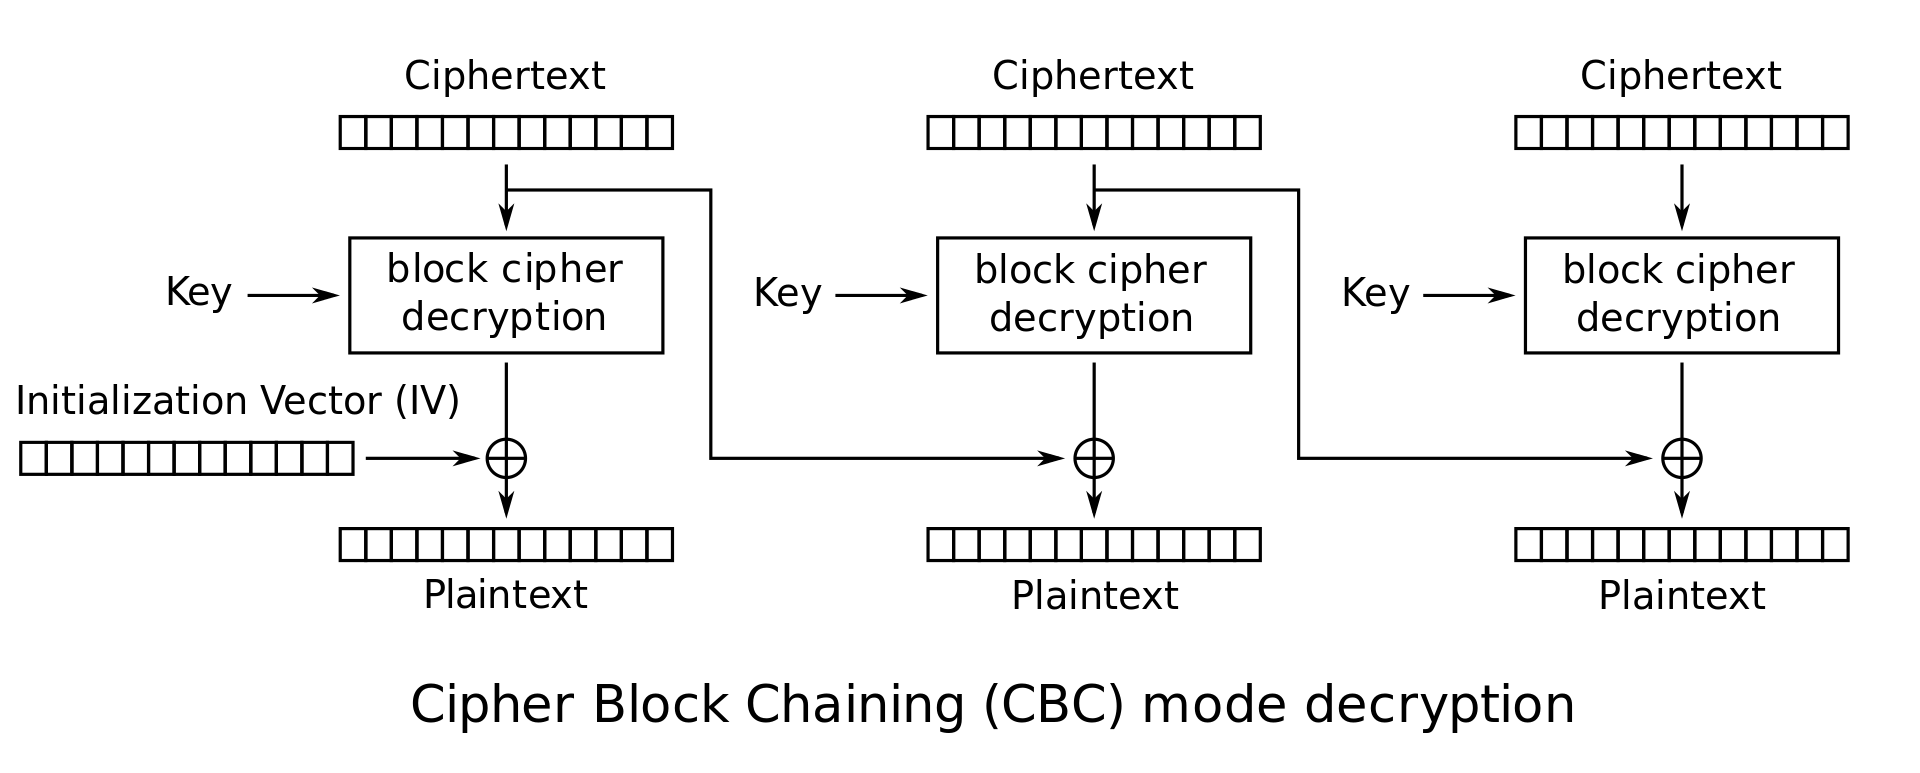
\includegraphics[width=12cm]{./Literatur/documents/CBC_decryption}\newline\caption{Entschlüsselung im CBC-Mode}
            \label{CBC_Mode_brechen}
        \end{center}
    \end{figure}


    \section{Sicherheitsbewertung}\label{sec:sicherheitsbewertung}
    Die schwachstelle Lucky 13 wird allgemein mit einer geringen Sicherheitsbewertungsstufe angegeben.
    Begründungen hierfür sind in erster Linie auch direkt die Erkennung des richtigen Paddings,welches über die Dauer der Antwort des Servers ermittelt wird.
    Das ist allerdings äußerst unwahrscheinlich, wenn man sich nicht im selben Netzwerk, wie der Server befindet.
    Nadhem J. AlFardan and Kenneth G. Paterson haben die Analysen für ihr Paper auch nur im selben Netzwerk durchgeführt.
    Suse schreibt dazu ``Please note that an exploit for this requires physical proximity of an attacker to the server, which is usually unlikely``, was Übersetzt bedeutet: Bitte beachten Sie, dass ein Exploit für dieses Problem die physische Nähe eines Angreifers zum Server erfordert, was in der Regel unwahrscheinlich ist.
    \newline
    Die Bewertung von Schwachstellen findet anhand des Common Vulnerability Scoring System (CVSS v2) statt, dies ist der Industriestandard zur Bewertung für mögliche und tatsächliche Sicherheitslücken.
    Dort werden verschiedene Kategorien, die in~\ref{tab:CVSS-Vektor} zusehen sind, bewertet und dann nach einer Formel ein Wert zwischen 0 und 10 ermittelt.
    Je geringer der Wert ist, desto kleiner ist das Risiko.
    Auf der Skala ist das Risiko bis 3,9 gering, zwischen 4,0 und 6,9 ist es medium und ab 7,0 ist das Risiko hoch.
    Deshalb wird von Suse der CVSS-Vector wie Folgt gesetzt:
    \begin{table}[h]
        \begin{tabular}{lllll}
        {\ul \textbf{Exploitability Metrics}}
            &         & & {\ul \textbf{Impact Metrics}}   & \multicolumn{1}{c}{} \\
            \textbf{Access Vector}     & Network & & \textbf{Confidentiality Impact} & Partial              \\
            \textbf{Access Complexity} & High    & & \textbf{Integrity Impact}       & None                 \\
            \textbf{Authentication}    & None    & & \textbf{Availability Impact}    & None
        \end{tabular}\caption{Bewertung von Lucky 13 durch Suse in der CVSS-Skalar (Version 2)}\label{tab:CVSS-Vektor}
    \end{table}
    \newline
    Das ergibt den Vektor AV:N/AC:H/Au:N/C:P/I:N/A:N mit einem CVSS-Score von 2.6.
    IBM bewertet Lucky 13 gleich, außer in Hinsicht auf die Access Complexity, die als medium gewertet wird, wodurch die Gesamtbewertung auf 4.3 ansteigt.
    Die beiden Bewertungen fallen gering aus, die von Suse ist im niedrigen Risiko und die von IBM im mittleren Bereich, wodurch zusagen ist, dass es unwahrscheinlich ist Opfer durch den Lucky 13 Angriff zu werden.


    \section{Gegenmaßnahmen}\label{sec:gegenmanahmen}
    Es gibt mehrere Maßnahmen, die ergriffen werden können, um einen Angriffserfolg zu minimieren.
    Die Maßnahmen müssen verhindern, dass man eine Zeitanalyse durchführen kann oder sie muss das benötigte Padding in der Blockverschlüsslung umgehen.

    \subsection{Zufällige Zeitverzögerungen}\label{subsec:zufallige-zeitverzogerungen}
    Bei einem Angriff, der auf die Dauer einer Reaktion abzielt, liegt eine zufällige verzögerung nahe.
    Allerdings ist dies ineffektiv wie N. AlFardan und K. G. Paterson schreiben~\cite[S.13]{AlFardan2013}.

    \subsection{Rons's Code 4 Chiffre}\label{subsec:rons's-code-4-chiffre}
    Die Ron's Code 4 Chiffre (RC4) wird zum bei der Veröffentlichung von N. AlFardan und K. G. Paterson als eine Möglichkeit zum Schutz erwähnt, weil kein Padding benötigt wird.
    Allerdings wurde auch gesagt, dass dies keine Möglichkeit für DTLS ist~\cite[S.13]{AlFardan2013}.
    2015 wurde von der Internet Engineering Task Force (IETF)  die Nutzung und Kommunikation über RC4 in verbindung mit TLS verboten, weil es Sicherheitsmängel aufweist.
    % https://www.rfc-editor.org/rfc/rfc7465

    \subsection{Implementierung der MEE-TLS-CBC-Entschlüsselung}\label{subsec:implementierung-der-mee-tls-cbc-entschlusselung}
    Dies ist die von den Publishern des Angriffs empfohlene Methode.
    Da bei geht es darum, die Verarbeitungszeit nicht von dem Inhalt oder dem Padding abhängig zu machen, sondern nur von der Länge der chiffrierten Nachricht \cite[s.13]{AlFardan2013}.
    Hier muss ich noch weiter schreiben.

    \newpage

    \bibliography{Literatur/Quellen}
\end{document}

